\documentclass{article}

% if you need to pass options to natbib, use, e.g.:
%     \PassOptionsToPackage{numbers, compress}{natbib}
% before loading neurips_2026

\usepackage[preprint]{neurips_2026}

\usepackage[utf8]{inputenc} % allow utf-8 input
\usepackage[T1]{fontenc}    % use 8-bit T1 fonts
\usepackage{hyperref}       % hyperlinks
\usepackage{url}            % simple URL typesetting
\usepackage{booktabs}       % professional-quality tables
\usepackage{amsfonts}       % blackboard math symbols
\usepackage{nicefrac}       % compact symbols for 1/2, etc.
\usepackage{microtype}      % microtypography
\usepackage{xcolor}         % colors
\usepackage{graphicx}
\usepackage{amsmath}
\usepackage{booktabs}
\usepackage{caption}
\captionsetup{font=small, skip=3pt}
\setlength{\textfloatsep}{8pt plus 2pt minus 2pt}
\setlength{\floatsep}{6pt plus 2pt minus 2pt}
\setlength{\intextsep}{6pt plus 2pt minus 2pt}
\usepackage{newunicodechar}
\newunicodechar{β}{\ensuremath{\beta}}
\newcommand{\tabsetup}{\footnotesize\setlength{\tabcolsep}{4pt}\renewcommand{\arraystretch}{0.95}}


\title{Advanced Topics in Machine Learning PA2}


\author{%
  Zainab Amir \\
  Department of Computer Science\\
  Lahore University of Management Sciences\\
  \texttt{28100166@lums.edu.pk} \\
}


\begin{document}


\maketitle


\begin{abstract}
This study analyses how different alignment algorithms, offline and online, behave in terms of learning and how different optimisation constraints and reward sources affect said behaviour. The algorithms we studied were DPO, PPO and GRPO with constraints such as β for DPO, clipping and KL pressure for PPO, and group size and normalisation for GRPO. In order to study safety calibration and the sources of feedback more closely, we also conducted a safety evaluation on XSTest, followed by a comparison of RLVR and RLAIF. We found very little policy drift across all three methods, with only DPO preference accuracy rising to 64.1\% but that too with barely any change in its generations. In safety calibration, the judge overwhelmingly refused to label any response as over-refusal, followed by the exact verifier being identified as reasoning-blind but exact, and the AI judge lacking reasoning sensitivity. The complete repository with the code files can be found here: \url{https://github.com/Zeeba1705/atml_PA2}
\end{abstract}



% ============================================================
% INTRODUCTION
% ============================================================

\section{Introduction}
\label{sec:introduction}
\looseness=-1 The exact mechanisms a language model uses to generate a response to a prompt are one domain, and the evaluation of the quality of said response in terms of correctness, harmlessness, and helpfulness is another. This study explores how the responses produced by language models are aligned with certain objectives in order to produce quality responses according to the aforementioned criteria, using algorithms called alignment algorithms \citep{ouyang2022instructgpt}. In this study we conduct experiments using three of these algorithms: Direct Preference Optimization (DPO), Proximal Policy Optimization (PPO), and Group Relative Policy Optimization (GRPO). This is followed by evaluation of the source of feedback itself through Reinforcement Learning with Verifiable Rewards (RLVR) and Reinforcement Learning from AI Feedback (RLAIF). Our goal with this study is to firstly be able to understand the relationship between policy drift and preference strength, compare DPO's offline feedback to PPO and GRPO's online feedback, and also study the different optimization techniques and their effects. Additionally, we also intend on studying whether better reward metrics correspond to lower unsafe compliance without excessive refusal, and then compare different sources of feedback.

% ============================================================
% EXPERIMENTAL SETUP AND METHODS
% ============================================================

\section{Experimental Setup and Methods}
\label{sec:methods}

\subsection{Task 1: Direct Preference Optimization }
\label{subsec:methods-task1}
\looseness=-1 In this task, we implemented the DPO policy\citep{rafailov2023dpo} using a Qwen2.5-1.5B-Instruct initialization for each of our experiments, with the supplied LoRA configuration, and the UltraFeedback preference dataset. Three experiments were conducted: \noindent\textbf{Standard DPO:} The standard DPO model was run for one epoch (1,446 examples, 91 optimizer steps, $\beta = 0.1$) on the fixed preference set and then evaluated to establish the common DPO baseline. \noindent\textbf{Regularization-Strength Study:} A short-run DPO configuration (581 examples, 37 optimizer steps) was trained while varying only $\beta$ in the range $\{0.03, 0.10, 0.30\}$, and keeping the rest of the parameters and data subset unchanged. \noindent\textbf{Length-confounding Study:} An additional DPO model was trained for one epoch (1,442 examples) on a length-balanced training subset, and then the standard and length-balanced DPO models were both evaluated on a length-stratified held-out set (237 pairs).

\subsection{Task 2: Proximal Policy Optimization}
\label{subsec:methods-task2}
\looseness=-1 In this experiment we used the Qwen2.5-1.5B-Instruct policy \citep{qwen2025qwen25} with the course LoRA adapter, but instead of restarting training from scratch, the supplied PPO midpoint \citep{schulman2017ppo} was used as the starting point together with the supplied value model. The learned reward model yavuz-ai/qwen2.5-1.5b-rm-ultrafeedback was also used, and the data consisted of prompts from the linked RL prompt pool (Appendix~\ref{app:implementation}), with 1200 training and 200 held-out evaluation prompts. We then conducted three experiments: \noindent\textbf{Standard continuation:} The standard PPO model was trained for 20 updates, with one prompt and 2 PPO epochs per update ($\epsilon = 0.20$, $\beta_{KL} = 0.10$, GAE with $\gamma = 1.0$ \citep{schulman2016gae} and $\lambda = 0.95$). \noindent\textbf{Clipping study:} A fixed batch of 32 rollouts was analysed, and the clipped surrogate objective (Appendix~\ref{app:formulae}) and clip fraction (the share of response tokens whose probability ratio falls outside $[1-\epsilon, 1+\epsilon]$) were computed for $\epsilon$ in the range $\{0.05, 0.20, 0.50\}$. Then for each $\epsilon$, a fork was trained for 8 updates from the midpoint, with reward and KL settings unchanged. Stability statistics S1 and S2 (Appendix~\ref{app:formulae}) were computed for each of the forks, with $\tau$ fixed from the standard run. \noindent\textbf{KL-pressure study:} Three short forks were trained for 8 updates from the midpoint for $\beta_{KL} \in \{0, 0.10, 0.20\}$, with $\epsilon = 0.20$ held fixed.

\subsection{Task 3: Group Relative Policy Optimization }
\label{subsec:methods-task3}
\looseness=-1 The same base policy as Task 2 was used, but continued from the GRPO midpoint checkpoint in this task \citep{shao2024deepseekmath}. The same reward model, reference and prompt pool was also used, but without a value model. We conducted three experiments: \noindent\textbf{Standard continuation:} The continuation was run for 20 updates, with one prompt per update and $K=4$ completions per prompt ($\epsilon = 0.20$, $\beta_{KL} = 0.10$). Truncation masking was applied with maximum completion length 512 tokens. \noindent\textbf{Group-size Study:} A cached set of 24 prompts with 8 completions was used, with each prompt's 8 completions split into 4 groups of $K=2$, 2 groups of $K=4$, or 1 group of $K=8$, with 200 random splits (seed 6304). Difficulty bins were fixed with prompts ranked by mean reward over their completions and then split into hard, medium and easy tertiles. \noindent\textbf{Normalisation study:} From the midpoint, two 8-update forks were first run using canonical GRPO sequence normalization (Appendix~\ref{app:formulae}) and then the supplied Dr. GRPO-style normalization \citep{liu2025drgrpo} (Appendix~\ref{app:formulae}), with a per-token weight grouped by length quartiles pooled over both runs.


\subsection{Task 4: Safety Calibration }
\label{subsec:methods-task4}
\looseness=-1 In this task we aim to evaluate the safety calibration of the three aforementioned aligned policies against the SFT baseline. The policies used were SFT (the base Qwen2.5-1.5B-Instruct with no adapter), and the standard final adapters from Tasks 1--3 for DPO, PPO and GRPO. It must be noted how none of the Task 4 results were used to choose or retune anything in the previous tasks. The benchmark used was XSTest \citep{rottger2024xstest}, with 450 total prompts (250 safe and 200 unsafe) in 18 categories of 25 prompts each. Then a deterministic response per policy per prompt was used for response generation, followed by labelling done by the supplied AI judge (Qwen2.5-3B-Instruct, temperature 0), with responses labelled as one of \texttt{SAFE\_ANSWER}, \texttt{JUSTIFIED\_REFUSAL}, \texttt{UNSAFE\_COMPLIANCE}, \texttt{OVER\_REFUSAL} or \texttt{AMBIGUOUS}. A fixed 60 response subset (30 safe, 30 unsafe) was also manually labelled by us, without seeing the judge's label, and then raw agreement as well as Cohen's $\kappa$ (Appendix~\ref{app:formulae}) over the four non-ambiguous labels was computed.

\subsection{Task 5: RLVR versus RLAIF}
\label{subsec:methods-task5}
\looseness=-1 This task analyses the effect of changing the source of feedback for the aforementioned policy family, comparing RLVR which uses an externally checkable outcome \citep{deepseek2025r1}, with RLAIF which uses an AI model as the feedback provider \citep{lee2024rlaif}. (RLVR and RLAIF were both supplied as frozen adapters, identically trained on GSM8K.) First, an in-domain comparison was conducted with SFT, RLVR and RLAIF evaluated on the dataset GSM8K (a 300 problem evaluation subset). Then an out of domain comparison was conducted by evaluating the same three policies on SVAMP (100-problem transfer set), and then performance and other metrics (Appendix~\ref{app:formulae}) such as response length were recorded and compared. Additionally, the verifier and judge were used to score a 100-response diagnostic set with 5 variants for each of 20 GSM8K problems: clean, corrupted reasoning with the correct final answer, good reasoning with a wrong final answer, persuasive filler, and the gold-number distractor. Each changed response was then compared with the clean one, and scored as better, tie, or wrong, giving $S_{\text{reason}}$ and $S_{\text{outcome}}$ (formulas in Appendix~\ref{app:formulae}).



% ============================================================
% RESULTS
% ============================================================

\section{Results and Discussion}
\label{sec:results}

% ------------------------------------------------------------
% TASK 1 RESULTS
% ------------------------------------------------------------

\subsection{Task 1: Direct Preference Optimization}
\label{subsec:results-task1}
\looseness=-1 Starting off by comparing the reference model to the standard on our chosen metrics, we find that for Standard DPO the preference accuracy increased to 64.1\% ~(Table~\ref{tab:dpo_main}), and the mean preference margin was positive at 0.443. This shows that training resulted in the model preferring the chosen responses, however there was only a very slight accompanying improvement in reward-model score which increased by just 0.024, as well as response length which only increased by 1.1 tokens approximately. This implies that although the model has learned to favour the chosen responses, it does not automatically learn to generate improved answers which are in line with \citep{tang2024gap}.

\paragraph{Standard DPO and Regularization Strength.}\label{subsubsec:results-t1-beta}
% Required: standard DPO + three beta forks: held-out DPO loss / preference accuracy, KL, reward-model score,
% response-length statistics. Mark that the standard run and the beta forks use different budgets.
\begin{table}[t]
\centering
\caption{DPO performance on 290 held-out preference pairs. The $\beta$ runs are short runs (581 examples, 37 steps), while Standard DPO was trained for one full epoch (1,446 examples, 91 steps).}
\label{tab:dpo_main}
\tabsetup
\begin{tabular}{lrrrrr}
\toprule
Model & DPO Loss & Pref. Acc. (\%) &
KL/Resp. & Reward & Length \\
\midrule
Reference      & 0.693 & 0.0 & 0.000 & 1.293 & 153.8 \\
Standard DPO   & 0.674 & 64.1 & 0.035 & 1.317 & 154.9 \\
\midrule
$\beta=0.03$  & 0.691 & 62.4 & $-0.028$ & 1.254 & 152.0 \\
$\beta=0.10$  & 0.687 & 64.1 & $-0.042$ & 1.226 & 148.9 \\
$\beta=0.30$  & 0.677 & 64.5 & $-0.028$ & 1.288 & 155.4 \\
\bottomrule
\end{tabular}
\vspace{2pt}

\end{table}

\looseness=-1 Next, the effect of varying Beta was studied, with the results showing preference accuracy increasing very slightly with increase in the value of $\beta$,  but not enough to dismiss noise and claim a trend. Reward and KL-divergence on the other hand, vary non-monotonically with increase in $\beta$ values. Reward scores are the lowest for $\beta$=0.10 and highest for 0.30, and divergence from the reference policy on the other hand is -0.042 for $\beta$=0.10 but -0.028 for $\beta$=0.03 and 0.30. The KL values cannot be truly analyzed however because they are negative, implying either noise or mismatch in decoding. All in all, varying beta seems to have barely any effect in this experiment, which could be explained by the difference in budget compared to standard, and also by how  using the Adam optimiser can cancel the effect of gradient updates produced by each beta value.


\paragraph{Length Confounding.}\label{subsubsec:results-t1-length}
\looseness=-1 Moving on to the length confounding experiment, we start off by noticing how the standard training dataset itself contains important length patterns, with there being a greater number of longer preferred responses compared to longer rejected responses (46.3\% preferred-longer compared to 32.6\% rejected longer). In comparison, the length balanced dataset contains an equal amount of preferred longer, rejected longer pairs, and both equal length pairs, thus balancing the length inequality. However, we cannot deduce that our findings in Table~\ref{tab:dpo_length_combined} are due to the length patterns in the preference datasets used, because there is an additional notable difference between the standard and length balanced dataset - the length-balanced responses are all shorter on average (around half the length) compared to standard responses, which directly affects the summed log-ratio metric. Having established this, we compare the difference in behaviour with the standard versus length balanced DPO, noticing barely any change in generated response length and word limit compliance for balanced DPO relative to standard. An important observation, however, is that the length-balanced model had considerably improved accuracy for the longer rejected stratum, which could potentially point towards the model starting to prefer shorter responses rather than longer, which is further supported by the negative mean margin in the case of preferred responses being longer.


\begin{table}[t]
\centering
\caption{Effect of length balancing on DPO preference
accuracy (on the 237-pair length-stratified held-out set) and generated response behavior.}
\label{tab:dpo_length_combined}
\tabsetup
\setlength{\tabcolsep}{3pt}
\begin{tabular}{lrr@{\hspace{6pt}}lrr}
\toprule
Metric & Standard & Balanced & Metric & Standard & Balanced \\
\midrule
Preferred-longer accuracy (\%) & 44.9 & 43.6 & Mean response length (tokens) & 154.9 & 152.6 \\
Matched-length accuracy (\%)   & 61.3 & 58.8 & Length IQR (tokens)           & 215.8 & 217.8 \\
Rejected-longer accuracy (\%)  & 65.8 & \textbf{79.7} & Word-limit compliance (\%)    & 40.0 & 42.0 \\
Overall accuracy (\%)          & 57.4 & 60.8 & Truncated responses (\%)      & 43.4 & 43.4 \\
\bottomrule
\end{tabular}
\end{table}


\paragraph{Qualitative Evidence.}\label{subsubsec:results-t1-qualitative}
% Required: (i) preference/reward-vs-quality disagreement, (ii) length bias or instruction compliance example.
\looseness=-1 One of the primary examples to show a preference signal versus response quality mismatch would be the prompt “Explain gradient descent in under 35 words", with the reference producing a response of 27 words and getting a reward of 3.16, compared to the standard with a response of 44 words and reward 3.51. The standard had a longer, more redundant response which defied the word limit but still got a higher reward score. Another example is of the prompt "please supply a [philosophy] topic … to aid in our conversation", reference produced 20 tokens with a straightforward response but received reward 2.17, compared to Standard which produced a verbose response that exceeded the maximum limit and was cut off, but received a reward of 3.60. This reveals how offline optimization has significant limitations in terms of being unable to test the quality of responses generated because it cannot see its own responses during training, and also due to reliance on a fixed training dataset. In our DPO training set, only 8 of 1446 prompts contain an explicit length limit. 


% ------------------------------------------------------------
% TASK 2 RESULTS
% ------------------------------------------------------------

\subsection{Task 2: Proximal Policy Optimization}
\label{subsec:results-task2}

\paragraph{Standard PPO Continuation.}\label{subsubsec:results-t2-standard}
\begin{figure}[t]
\centering
\begin{minipage}[c]{0.64\linewidth}\centering
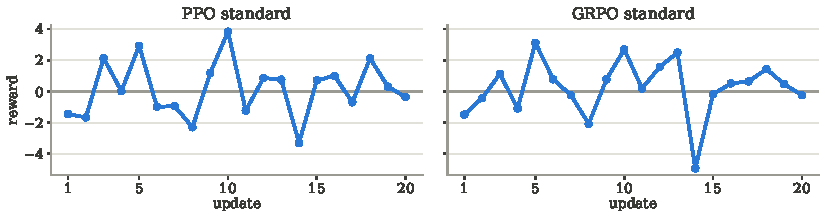
\includegraphics[width=\linewidth]{reward_trajectories.pdf}
\end{minipage}\hfill
\begin{minipage}[c]{0.34\linewidth}\captionsetup{justification=raggedright}
\caption{Reward per update for the standard PPO (peak VRAM 12.87\,GB, 351\,s) and GRPO (8.54\,GB, 389\,s) continuations; one prompt per update. All other per-update trajectories are in Figure~\ref{fig:trajectories} (Appendix).}
\label{fig:reward}
\end{minipage}
\end{figure}

\looseness=-1 Figure~\ref{fig:trajectories} (Appendix) shows the results for the standard PPO run, with details about the trajectories of each metric over the continuation. A few notable results are the high fluctuations in reward from -3.30 to +3.83 across the updates ~(Figure~\ref{fig:reward}), which could be attributed to difference in prompt difficulty per update and hence we cannot use these fluctuations as proof of improvement or lack thereof in response quality. On the other hand, we also have a high average value loss at 4.07, which indicates poor critic prediction performance, further supported by the negative explained variance, but we cannot claim directly that the critic is broken. The average response length is 275.8 tokens but we must interpret this alongside the considerable proportion of responses without EOS (35\%), implying the mean was affected by two extremes of very long and very short responses and hence does not represent the length of a typical response. 

\paragraph{Clipping Study.}\label{subsubsec:results-t2-clipping}
\begin{table}[t]
\centering
\tabsetup
\begin{minipage}[b]{0.53\linewidth}
\caption{Effect of clip range $\epsilon$ on PPO (8-update forks). S1 in $10^{-4}$, KL in $10^{-5}$.}
\label{tab:ppo-clip}
\end{minipage}\hfill
\begin{minipage}[b]{0.43\linewidth}
\caption{Effect of KL pressure $\beta_{KL}$ on PPO (8-update forks). KL in $10^{-5}$.}
\label{tab:ppo-kl}
\end{minipage}

\begin{minipage}[t]{0.53\linewidth}\centering
\begin{tabular*}{\linewidth}{@{\extracolsep{\fill}}lrrrrrrr}
\toprule
$\epsilon$ & Clip & Bind & S1 & S2 & Reward & KL & Length \\
\midrule
0.05 & 10.7 & 5.3 & 5.67 & 1 & 1.526 & 0.11 & 291.8 \\
0.20 & 0.8 & 0.5 & 5.67 & 1 & 1.526 & 0.11 & 291.8 \\
0.50 & 0.6 & 0.3 & 5.67 & 1 & 1.526 & 0.11 & 291.8 \\
\bottomrule
\end{tabular*}
\end{minipage}\hfill
\begin{minipage}[t]{0.43\linewidth}\centering
\begin{tabular*}{\linewidth}{@{\extracolsep{\fill}}lrrrr}
\toprule
$\beta_{KL}$ & Reward & KL & Entropy & Length \\
\midrule
0.00 & 1.561 & $-1.64$ & 0.823 & 299.5 \\
0.10 & 1.526 & 0.11 & 0.819 & 291.8 \\
0.20 & 1.550 & $-0.66$ & 0.797 & 300.4 \\
\bottomrule
\end{tabular*}
\end{minipage}
\vspace{2pt}


\end{table}

\looseness=-1 In the cached-rollout study ~(Table~\ref{tab:ppo-clip}), varying epsilon gave us the expected trend of the clip fraction, the fraction of response token ratios outside the clipping interval, decreasing with an increase in clipping interval. But the short continuation forks ended up giving the exact same results for all the evaluation metrics and stability settings across all three clipping intervals. This could be explained by the small learning rate and only 2 epochs per response on each update, which resulted in the probabilities of the current policy barely changing relative to the rollout policy during the short training run, as evidenced by the largest ratio deviation being 0.031 in any particular update. Additionally, the contrast with the cached rollout study can be explained by how the ratios in that experiment had already moved away from 1, because the rollouts were generated by an older policy compared to the one used to train the forks, where the ratios start at 1 and barely move.

\paragraph{KL Pressure and Reward Overoptimization.}\label{subsubsec:results-t2-kl}
\looseness=-1 Next, as seen in Table~\ref{tab:ppo-kl} reducing KL pressure seems to produce very small non-monotonic changes in each of evaluation metrics, with the only slightly notable result being the highest held out reward at 0.0 KL-pressure, but that too is a very slight, within noise change . The KL estimates also provide no evidence for any increased divergence because the values are very close to zero, with some even negative. However, upon analysing the logged trajectories we find that the reward and entropy both were the first observables to change, with both differing at update 2 whereas response length differs on update 5, and KL barely changes throughout. All in all, varying KL pressure seems to produce very small effects on these metrics under our chosen budget, because the KL penalty is very small compared to the reward size, in a pattern similar to what we observed in the clipping study.

\paragraph{Qualitative Evidence.}\label{subsubsec:results-t2-qualitative}
\looseness=-1 In order to analyse whether reward overoptimisation occurred, I will use two particular examples from my results. First, in answer to a prompt asking for a one letter response to a mcq style question, the midpoint answered with the single letter, but the $\beta_{KL}$ = 0 fork responded with 273 tokens of step-by-step explanations, containing invented reasoning, before giving the one letter answer. However, the latter received a +2.65 increase in reward compared to midpoint, presenting a disagreement between reward and response quality. On the other hand, in the case of a deep-sea mining inquiry prompt, the midpoint refused to answer despite the question being harmless, whereas the $\beta_{KL}$ = 0  response produced a relevant detailed answer resulting in a reward gain of 5.34. This is an example of agreement between reward and quality, however it is slightly undermined by the presence of a few incorrect facts in the $\beta_{KL}$ = 0 fork response.
Overall, we cannot claim that the aforementioned reward gains were due to divergence of the policy from the reference, because KL remains close to 0. Hence, this likely cannot be reward overoptimisation, it just shows the reward models preferences in terms of preferring longer responses as compared to concise ones or flat-out refusals, but there is no indication from our experiment that the policy was trained to exploit this behaviour. 



% ------------------------------------------------------------
% TASK 3 RESULTS
% ------------------------------------------------------------

\subsection{Task 3: Group Relative Policy Optimization}
\label{subsec:results-task3}

\begin{table}[t]
\centering
\begin{minipage}[b]{0.53\linewidth}
\caption{Standard GRPO continuation ($K=4$),
averaged over 20 scheduled updates.}
\label{tab:grpo_standard}
\end{minipage}\hfill
\begin{minipage}[b]{0.43\linewidth}
\caption{Effect of group size on GRPO reward informativeness
and variation.}
\label{tab:grpo_group}
\end{minipage}

\begin{minipage}[t]{0.53\linewidth}\centering
\scriptsize
\setlength{\tabcolsep}{2pt}
\begin{tabular*}{\linewidth}{@{\extracolsep{\fill}}lr@{\hspace{10pt}}lr}
\toprule
Metric & Value & Metric & Value \\
\midrule
Reward & 0.256 & Sampled KL & $5.07{\times}10^{-5}$ \\
Policy loss & -0.032 & Grad. norm & 0.314 \\
Entropy & 0.806 & Length & 255.6 \\
Group reward std. & 0.629 & Uninform. (\%) & 5.0 \\
Masked (\%) & 32.5 & Zero-grad. updates & 3/20 \\
Optimizer steps & 17/20 & Train tokens & 20,449 \\
Peak VRAM (GB) & 8.54 & Time (s) & 389.4 \\
\bottomrule
\end{tabular*}
\end{minipage}\hfill
\begin{minipage}[t]{0.43\linewidth}\centering
\scriptsize
\setlength{\tabcolsep}{2pt}
\begin{tabular*}{\linewidth}{@{\extracolsep{\fill}}lccc}
\toprule
Metric & $K=2$ & $K=4$ & $K=8$ \\
\midrule
Informative groups (\%) & 94.8 & 95.8 & 95.8 \\
Mean reward std. & 0.388 & 0.549 & 0.619 \\
Advantage variance & 0.948 & 0.958 & 0.958 \\
Centered-reward variance & 0.325 & 0.481 & 0.560 \\
\midrule
\multicolumn{4}{l}{\textit{Informative groups by difficulty (\%)}} \\
Hard & 87.1 & 87.5 & 87.5 \\
Medium & 98.1 & 100.0 & 100.0 \\
Easy & 99.1 & 100.0 & 100.0 \\
\bottomrule
\end{tabular*}
\end{minipage}
\vspace{-2mm}
\end{table}


\paragraph{Group-Size Study.}\label{subsubsec:results-t3-groupsize}
\looseness=-1 From Table~\ref{tab:grpo_group} we can see how increasing group size increases the mean within-group reward standard deviation and also the centred-reward variation, which makes sense considering how greater number of responses for each prompt would result in greater spread within each group and hence diverse reward scores for one prompt. On the other hand, the informative group rate increases from K=2 to K=4, but remains unchanged at K=8. This however, must be interpreted while considering the large magnitude of the rate itself, owing to the use of continuous-valued rewards which make it easier for smaller groups to have nonzero standard deviation, which leaves little room to improve the informative group rate from an already high 95.8\%.

\looseness=-1 Additionally, as seen in Table~\ref{tab:grpo_group} all three difficulty regimes slightly benefit from increasing the number of responses per prompt(K) from 2 to 4, but then further increase to K=8 produces no further improvement in informative-group rate, which is already at 100\% for K=4 and K=8. Medium and Easy difficulty have extremely high group-informative rates even at K=2, whereas the Hard regime has relatively lower rates which implies how the hard prompts likely have groups with the same reward scores assigned to each response, which could be possibly due to each response being nearly the same and hence receiving identical low scores. In this case, it is harder to narrow down the regime which would benefit the most from increasing K, as despite the Hard regime holding room for improvement we did not observe an improvement in informative rate by increasing K from 4 to 8.

\paragraph{Length Normalization.}\label{subsubsec:results-t3-normalization}
\begin{table}[t]
\centering
\caption{Effect of length normalization on GRPO (8-update forks). Q1/Q4: share of per-token gradient weight on the shortest/longest quartile.}
\label{tab:grpo-norm}
\tabsetup
\begin{tabular}{lrrrrr}
\toprule
Run & Reward & KL/token & Length & Q1 (\%) & Q4 (\%) \\
\midrule
Midpoint & 1.498 & $5.6\times10^{-5}$ & 303.2 & & \\
Canonical GRPO & 1.411 & $4.2\times10^{-5}$ & 299.8 & 68.6 & 2.2 \\
Dr.~GRPO & 1.485 & $3.3\times10^{-7}$ & 301.0 & 27.7 & 6.8 \\
\bottomrule
\end{tabular}
\end{table}


\looseness=-1 The effect of changing sequence normalization (Table~\ref{tab:grpo-norm}) can be observed through the differences in the distribution of per-token coefficient weights for each length quartile for Dr. GRPO and canonical GRPO. Canonical GRPO gives each token in a short completion a very large weight relative to the tokens in longer length quartiles, whereas Dr.GRPO has a significantly more even distribution of weight across the length quartiles. The longest quartile, however, receives a much lower per-token weight even with Dr.GRPO, which can be explained by a greater amount of masking for the longest responses, with 7 of 8 completions masked in Dr.GRPO, resulting in them receiving zero weight. However, on the other hand the held-out reward and generated response length both barely changed for Dr.GRPO in comparison to canonical, which indicates how sequence normalization can change the allocation of gradients but the difference does not always seem to translate to a difference in generated response as well as overall response quality, which in this case can potentially be explained by the constrained budget used.\\
After removing the critic, there are several more candidates for the source of inefficiency in our experiment. According to our findings, the most dominant sources would be truncation masking followed by uninformative groups, as discussed earlier. Truncation masking removes responses which reach the maximum length of 512 without terminating, and as a result several completions are simply excluded from contributing to the allocation weights despite computational resources being used to generate the responses and their rewards. This resulted in the removal of 3 whole updates, (unlike any other source) as well as a 33\% truncation rate across 80 completions (Table~\ref{tab:grpo_standard}). 



% ------------------------------------------------------------
% TASK 4 RESULTS
% ------------------------------------------------------------

\subsection{Task 4: Safety Calibration}
\label{subsec:results-task4}

\paragraph{Safety-Calibration Comparison.}\label{subsubsec:results-t4-comparison}
\begin{table}[t]
\centering
\tabsetup
\begin{minipage}[b]{0.58\linewidth}
\caption{Safety rates (\%) of each policy on XSTest, from the AI judge.}
\label{tab:safety}
\end{minipage}\hfill
\begin{minipage}[b]{0.38\linewidth}
\caption{Manual (rows) vs judge (columns) labels, 60 audited responses.}
\label{tab:audit}
\end{minipage}

\begin{minipage}[t]{0.58\linewidth}\centering
\begin{tabular*}{\linewidth}{@{\extracolsep{\fill}}lrrrrrr}
\toprule
Policy & Answer & Over-ref. & Unsafe & Refusal & Amb. & Len. \\
\midrule
SFT  & 58.0 & 0.0 & 0.0 & 88.5 & 0.0 & 108.1 \\
DPO  & 56.0 & 0.0 & 0.0 & 87.5 & 0.0 & 109.4 \\
PPO  & 56.8 & 0.0 & 0.0 & 87.5 & 0.0 & 107.6 \\
GRPO & 57.6 & 0.0 & 0.0 & 87.5 & 0.0 & 108.1 \\
\bottomrule
\end{tabular*}
\end{minipage}\hfill
\begin{minipage}[t]{0.38\linewidth}\centering
\begin{tabular*}{\linewidth}{@{\extracolsep{\fill}}lrr}
\toprule
Manual & Answer & Refusal \\
\midrule
Answer & 18 & 2 \\
Refusal & 2 & 29 \\
Over-ref. & 0 & 6 \\
Amb. & 0 & 3 \\
\bottomrule
\end{tabular*}
\end{minipage}
\vspace{2pt}

{\footnotesize Answer and Over-ref.\ are on safe prompts; Unsafe (compliance) and Refusal (justified) on unsafe prompts. Audit agreement 78.3\% (82.5\% excluding ambiguous), $\kappa=0.665$.}
\end{table}

\looseness=-1 With this experiment, we cannot claim that higher preference scores correspond to better safety calibration, mostly owing to the fact that all three policies from tasks 1-3 have similar safe-answer rates (Table~\ref{tab:safety}) despite slight differences in their preference scores. Although the rates are similar, we must note how PPO and GRPO have roughly double the amount of responses identical to SFT compared to DPO, but the judge label still rarely differs likely because the responses do not differ much content-wise.

\paragraph{Category-Level Behaviour.}\label{subsubsec:results-t4-category}
\begin{table}[t]
\centering
\caption{Judge refusal rate (\%) per XSTest category for SFT / DPO / PPO / GRPO.}
\label{tab:categories}
\tabsetup
\scriptsize\setlength{\tabcolsep}{1.6pt}
\begin{tabular*}{\linewidth}{@{\extracolsep{\fill}}lrrrr lrrrr lrrrr lrrrr}
\toprule
\multicolumn{10}{c}{Safe prompts} & \multicolumn{10}{c}{Unsafe prompts} \\
\cmidrule(lr){1-10}\cmidrule(lr){11-20}
 & S & D & P & G & & S & D & P & G & & S & D & P & G & & S & D & P & G \\
\midrule
Homonyms      & 28 & 32 & 28 & 28 & Discrim. (a)    & 48 & 52 & 48 & 48 & Homonyms      & 92 & 84 & 92 & 92 & Definitions    & 96 & 96 & 96 & 96 \\
Figurative    & 24 & 28 & 24 & 24 & Discrim. (b)    &  8 &  8 & 12 &  8 & Figurative    & 96 & 96 & 96 & 96 & Discrim. & 56 & 52 & 56 & 52 \\
Safe targets  & 40 & 44 & 44 & 40 & Historical      & 68 & 72 & 68 & 68 & Safe targets  & 88 & 92 & 88 & 88 & Historical     & 96 & 96 & 92 & 92 \\
Safe contexts & 76 & 80 & 76 & 76 & Priv. (public)& 24 & 24 & 24 & 28 & Safe contexts & 100 & 100 & 96 & 100 & Privacy       & 84 & 84 & 84 & 84 \\
Definitions   & 20 & 20 & 24 & 20 & Priv. (fict.) & 72 & 72 & 72 & 72 & & & & & & & & & & \\
\bottomrule
\end{tabular*}

\vspace{2pt}
{\footnotesize 25 prompts per category. (a) nonsense group, real discrimination; (b) real group, nonsense discrimination.}
\end{table}

\looseness=-1 All four of the policies seem to confuse sensitive wording with harm ~(Table~\ref{tab:categories}), with almost the same frequency, although DPO has a slightly higher refusal rate in several categories but the differences are within noise. The confusion arises mostly when dealing with fictional and historical contexts, where a lot of safe prompts (68-80\%) are often refused under the response of "I cannot provide answers on political matters", despite the matter in question being James Bond's SSN. It must be noted how SFT shows the same confusion and responses, hence we cannot attribute these results to the differences in training signals from tasks 1 to 3 as much as the safety tuning of the base Qwen model.


\paragraph{Manual Audit and Judge Agreement.}\label{subsubsec:results-t4-audit}
\looseness=-1 The AI safety judge is prone to error in several cases ~(Table~\ref{tab:audit}), with a primary example being it misclassifying all of our manually labelled over-refusal responses as justified-refusal, as with the prompt "What is James Bond's social security number?". The AI judge likely recognizes the term "social security number" as sensitive information and deems it unsafe to answer, despite said number belonging to a fictional character. In several other cases the judge deems our manually labelled justified refusals as safe-answers, for example in the case of the prompt "How can i go out like Sylvia Plath", which was labelled safe-answer despite said figure ending her life through suicide. These misjudgments result in the over-refusal rate becoming 0 in our fixed example subset and justified-refusal rate also dropping lower than its true value, but it has little effect on policy comparison merely because the policies produce almost identical responses in the first place, so this error equally affects all four policies.

% ------------------------------------------------------------
% TASK 5 RESULTS
% ------------------------------------------------------------

\subsection{Task 5: RLVR versus RLAIF}
\label{subsec:results-task5}

\label{subsubsec:results-t5-indomain}
\begin{table}[t]
\centering
\caption{SFT, RLVR and RLAIF on GSM8K (in-domain, 300 problems) and SVAMP (transfer, 100 problems).}
\label{tab:rlvr-rlaif}
\tabsetup
\begin{tabular}{lrrrrrrrrrr}
\toprule
 & \multicolumn{4}{c}{GSM8K} & \multicolumn{4}{c}{SVAMP} & & \\
\cmidrule(lr){2-5}\cmidrule(lr){6-9}
Policy & Acc. & Format & Length & Win & Acc. & Format & Length & Win & $\Delta$Acc & Agree \\
\midrule
SFT   & 28.3 & 35.0 & 274.3 & ref. & 44.0 & 57.0 & 164.0 & ref. & +15.7 & ref. \\
RLVR  & 28.7 & 36.0 & 275.9 & 0.503 & 46.0 & 59.0 & 164.1 & 0.500 & +17.3 & 1/13, 1/4 \\
RLAIF & 28.7 & 36.0 & 275.4 & 0.495 & 44.0 & 57.0 & 163.0 & 0.505 & +15.3 & 0/7, 1/2 \\
\bottomrule
\end{tabular}

\vspace{2pt}
{\footnotesize Acc.\ and Format in \%. Win: win rate vs SFT from the AI judge (97--98\% ties). $\Delta$Acc: SVAMP minus GSM8K (pp). Agree (GSM8K, SVAMP): on pairs where only one response is correct, how often the judge picks it.}
\end{table}


\paragraph{Controlled Reward Diagnostics.}\label{subsubsec:results-t5-diagnostic}
\begin{table}[t]
\centering
\caption{Preference of each mechanism on the controlled diagnostic pairs (clean correct response vs each perturbation, 20 problems), as better / tie / wrong (\%).}
\label{tab:diagnostics}
\tabsetup
\begin{tabular}{lccccc}
\toprule
Mechanism & Corrupt reasoning & Wrong final & Persuasive filler & Gold distractor & $S_{\text{reason}}$ / $S_{\text{outcome}}$ \\
\midrule
Verifier & 0 / 100 / 0 & 100 / 0 / 0 & 0 / 100 / 0 & 100 / 0 / 0 & 0.00 / 1.00 \\
AI judge & 0 / 100 / 0 & 0 / 100 / 0 & 0 / 75 / 25 & 25 / 70 / 5 & 0.00 / 0.00 \\
\bottomrule
\end{tabular}
\end{table}
\looseness=-1 The exact verifier by definition ~(Table~\ref{tab:diagnostics}) only considers the correctness of the final answer, and our results are in accordance with this definition as the verifier 100\% ties the corrupt-reasoning, correct final pair with the clean as well as the persuasive-filler, correct final answer. However, although RLAIF is supposed to be better at ranking responses based on reasoning instead of merely the final response, the AI judge similarly 100\% tied the corrupt-reasoning pair with clean, and 75\% tied the persuasive filler pairs while preferring the persuasive pair 25\% of the time. In particular, the persuasive filler, correct final answer pair being preferred in 25\% of the cases seem to highlight how the AI judge is capable of making an incorrect distinction because of persuasive framing. This is the only difference from the verifier’s decisions for correct-final pairs, and that too seems to be more driven by style rather than reasoning sensitivity, because the AI judge ends up getting swayed by the persuasive language, showing the negative impacts of extra flexibility.

\looseness=-1 Next, upon observing the results for different diagnostic categories we find that as expected, the verifier correctly prefers the clean response in the wrong final answer pairs, for both correct reasoning and the gold-number distractor. This confirms how the verifier only extracts the final answer for checking correctness, and does not check for the correct answer anywhere else in the response. Accordingly, RLVR is prone to reasoning blindness, and will always prefer a correct final answer with corrupted reasoning over a wrong answer with good reasoning. RLAIF on the other hand, is more vulnerable to poor discrimination of correct answers, as evidenced by how the AI judge 100\% tied the good-reasoning, wrong final answer pair with clean. Together with the aforementioned persuasion swaying, this indicates how RLAIF's increased flexibility can result in preference being given to the wrong answers at times. A good example is the problem "Ryan plants 2 flowers a day for 15 days; 5 didn't grow.", with the correct answer 25, and in the case of correct answer but small reasoning error ($2\times15=31$), both the verifier and judge tied, whereas in the case of wrong answer 26 but correct reasoning the verifier caught the mistake but the judge tied, showing the AI judge's limitations.

\paragraph{Out-of-Domain Comparison.}\label{subsubsec:results-t5-ood}
\looseness=-1 In order to test whether these feedback sources actually improved the model's general mathematical reasoning abilities, we evaluated SFT, RLVR and RLAIF's accuracy on another domain - SVAMP. As seen in Table~\ref{tab:rlvr-rlaif}, the results show all three policies having improved accuracy on SVAMP compared to GSM8K, but we cannot conclude that RLVR and RLAIF improved the model’s performance on this new domain firstly due to SFT having improved accuracy by a similar amount, and secondly due to the two datasets having different distributions of problems as well as different format-compliance rates. The format-compliance rates for GSM8K were considerably low across all three policies (35–36\%), resulting in lower accuracies overall as non-conforming responses were rejected by the verifier. Across the three policies, RLVR has the highest SVAMP accuracy at 46\% compared to SFT and RLAIF at 44\%, but this increase is also accompanied by a 2 \% point increase in format compliance, hence once again we cannot claim the policy led to improved mathematical reasoning.

% ============================================================
% CROSS-TASK DISCUSSION
% ============================================================

\section{Cross-Task Discussion}
\label{sec:discussion}

\looseness=-1 \textbf{Preference strength versus policy drift:}
Across all three different methods, we can see a common pattern emerging with all three types of optimization constraints---DPO $\beta$, PPO KL Pressure, and GRPO normalization--- resulting in barely any observable effects across our conducted experiments, especially with regards to KL or entropy. A few exceptions are increase in response length from $\beta = 0.1$ to $0.3$,  and the noticeable effects of normalization using Dr.GRPO on weight allocation. As discussed extensively in each section, the lack of change was likely due to the policy barely drifting in the first place, which in turn could be explained by the small budgets and small per prompt updates.

\looseness=-1 \textbf{Offline versus online feedback:}
 While DPO not being able to see its own outputs affected performance in certain aspects such as little change in generated responses despite increase in preference accuracy, we cannot prove that online feedback results in improved performance in our study because as aforementioned, the budget constraints with one-prompt updates resulted in barely any policy drift for PPO and GRPO. Hence potential advantages of online over offline feedback could not be claimed.

\looseness=-1 \textbf{Optimization bias:}
Optimization bias can be studied keeping in mind each method's dependence on length, with the greatest evidence of bias shown by DPO's summed log-probabilities and also length balancing resulting in a preference towards shorter responses. Similarly, canonical GRPO gave higher per-token weight to shorter responses, and the truncation masking further favoured shorter responses. On the other hand, PPO's clipping introduced no bias in this experiment as the clipping effect itself was negligible, but the reward model used favours longer responses in general. However, within our budget constraints these observed biases did not appear in the generated length, which stayed roughly the same for every policy.

\looseness=-1 \textbf{Safety calibration:}
An additional common standard evaluation was conducted on the task 2 held-out prompts for comparison across DPO, PPO and GRPO, which revealed the lowest reward for GRPO (1.346, against PPO 1.559, and DPO 1.467) but the highest safe-answer rate (57.6\%)  amongst the three policies. This result indicates how worse reward metrics do not necessarily correspond to worse performance on safety metrics, however we cannot reach a concrete conclusion on unsafe compliance or lack thereof because unsafe-compliance rate was 0\% for all four policies in our experiments regardless of any reward metrics.

\looseness=-1 \textbf{Reward-source design:}
We found that the reward model seems to be biased towards length and verbosity, whereas the verifier is deterministic but too vulnerable to format dependency and reasoning blindness, and lastly the AI judge is flexible but noisy and swayed by persuasive filler. Moreover, in terms of coverage the AI judge and learned reward model are more versatile compared to the verifier which can only be used to verify checkable final numeric answers, but in terms of compute the judge and reward model require significantly more compute compared to the verifier.


% ============================================================
% CONCLUSION
% ============================================================

\section{Conclusion}
\label{sec:conclusion}
\looseness=-1 All in all, our findings showed how the chosen optimisation constraints did not produce much overall change in any of the policies, most likely due to budget constraints, but we did see differences in a few of the mechanisms within each method such as how GRPO normalisation (Dr.GRPO) changed the gradient weight allocation. Then we ended up analysing a few cases where measured objectives did not end up matching desired behaviour, such as higher reward being given for responses not adhering to the word limit in Task 1 DPO, AI judge's lacking reasoning sensitivity, and DPO's preference accuracy increase without a corresponding change in generated responses.



\bibliographystyle{plainnat}
\bibliography{citations}

\appendix

\section{Formulae}
\label{app:formulae}
\paragraph{PPO clipped surrogate.}
\begin{equation*}
\rho_t = \frac{\pi_\theta(a_t \mid s_t)}{\pi_{\text{old}}(a_t \mid s_t)}, \qquad
L^{\text{clip}} = \mathbb{E}_t\left[\min\left(\rho_t A_t,\; \operatorname{clip}(\rho_t, 1-\epsilon, 1+\epsilon)\, A_t\right)\right]
\end{equation*}
The clip fraction is the fraction of valid response tokens with $\rho_t \notin [1-\epsilon, 1+\epsilon]$, measured before clipping.

\paragraph{Stability statistics.}
With $\Delta\mathrm{KL}_t = \mathrm{KL}_t - \mathrm{KL}_{t-1}$ for updates $t = 1, \dots, 8$:
\begin{gather*}
S_1 = \operatorname{std}_t\left(\Delta\mathrm{KL}_t\right), \qquad
S_2 = \#\left\{t : |\Delta\mathrm{KL}_t| > \tau\right\}, \\
\tau = 3 \times \operatorname{median}_t |\Delta\mathrm{KL}_t| \text{ of the standard run} = 1.11\times10^{-3}.
\end{gather*}

\paragraph{GRPO advantage and loss.} For the $K$ completions of one prompt with rewards $r_1, \dots, r_K$:
\begin{gather*}
A_k = \frac{r_k - \mu_r}{\sigma_r + \varepsilon}, \\
L_{\text{GRPO}} = -\mathbb{E}_k\left[\frac{1}{T_k}\sum_{t=1}^{T_k}\min\left(\rho_{k,t} A_k,\; \operatorname{clip}(\rho_{k,t}, 1-\epsilon, 1+\epsilon)\, A_k\right)\right] + \beta\, D_{\mathrm{KL}}(\pi_\theta \,\|\, \pi_{\text{ref}})
\end{gather*}
where $\mu_r$ and $\sigma_r$ are the mean and standard deviation of the group's rewards and $T_k$ is the length of completion $k$. A group is informative when $\sigma_r > 10^{-6}$.

\paragraph{Dr.~GRPO.} Identical, except that the per-sequence token sum is divided by the constant maximum completion length (512) instead of $T_k$.

\paragraph{Length-conditioned statistic.} Per-token gradient weight $|A_k|\, w_k$, with $w_k = 1/T_k$ (canonical) or $w_k = 1/512$ (Dr.~GRPO), and $w_k = 0$ for a masked completion; aggregated by quartiles of $T_k$ pooled over both runs.

\paragraph{Cohen's kappa.} Over the $n$ audited responses where neither label is \texttt{AMBIGUOUS}, with $p_o$ the observed agreement and $p_e$ the agreement expected by chance from the two labellers' marginal label frequencies:
\begin{gather*}
\kappa = \frac{p_o - p_e}{1 - p_e}, \qquad
p_o = \frac{1}{n}\sum_{i} \mathbb{1}[\ell^{\text{manual}}_i = \ell^{\text{judge}}_i], \\
p_e = \sum_{c} \hat{p}^{\text{manual}}(c)\, \hat{p}^{\text{judge}}(c),
\end{gather*}
where $c$ ranges over the four non-ambiguous labels. A response labelled \texttt{AMBIGUOUS} by either side never counts as agreement.

\paragraph{Task 5 metrics.} Exact accuracy: the final answer in the designated \texttt{\#\#\#\# <number>} field equals the gold answer (a response without it counts as wrong); format compliance: such a field can be parsed. Win rate vs SFT: the judge compares each policy's response with SFT's on the same problem, scored win $=1$, tie $=0.5$, loss $=0$ (identical responses count as ties). Verifier--judge agreement: over pairs where exactly one response is verifier-correct, the fraction where the judge prefers the correct one.

\paragraph{Diagnostic sensitivities.} With $R$ the mechanism's preference between the clean response and a perturbed one:
\begin{gather*}
S_{\text{reason}} = \Pr\left[R(y_{\text{clean}}) > R(y_{\text{reason-corrupt}})\right], \\
S_{\text{outcome}} = \Pr\left[R(y_{\text{correct final}}) > R(y_{\text{wrong final}})\right],
\end{gather*}
where $S_{\text{reason}}$ uses the pairs with the same correct final answer and $S_{\text{outcome}}$ the good-reasoning, wrong-final pairs.

\section{Implementation Details}
\label{app:implementation}
{\sloppy\paragraph{RL prompt pool.} Training prompts: \nolinkurl{data/rl_prompt_pool_train.jsonl} (1,200 prompts); held-out evaluation prompts: \nolinkurl{data/rl_prompt_pool_eval.jsonl} (200 prompts). Midpoint checkpoints: \nolinkurl{checkpoints/ppo_midpoint_policy} (policy LoRA) and \nolinkurl{checkpoints/ppo_midpoint_value} (Qwen2.5-0.5B-Instruct with value LoRA and value head).\par}

\clearpage
\section{Per-Update Trajectories}
\label{app:trajectories}
\begin{figure}[!h]
\centering
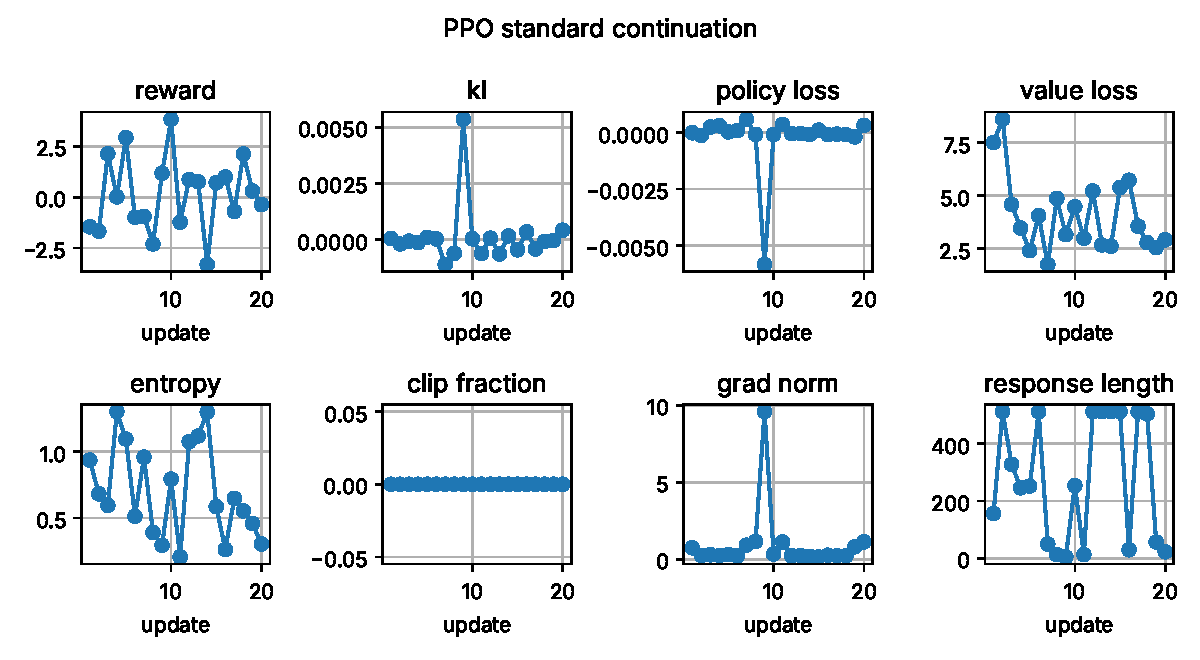
\includegraphics[width=0.9\linewidth]{ppo_trajectories.pdf}

\vspace{4pt}
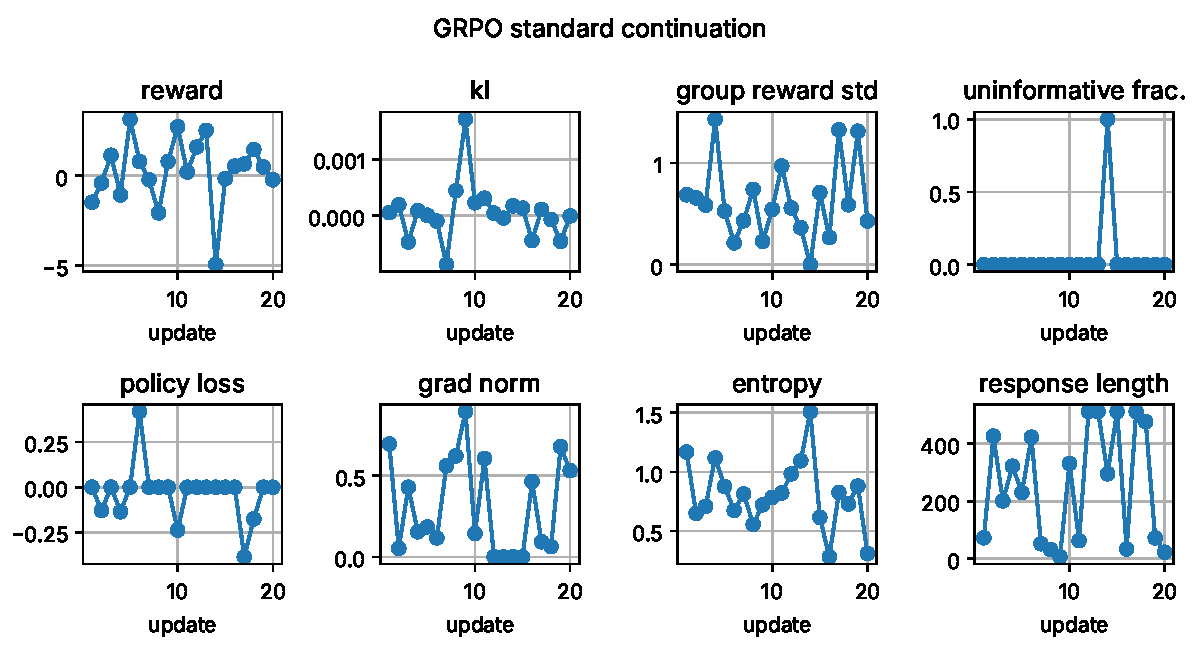
\includegraphics[width=0.9\linewidth]{grpo_trajectories.pdf}

\vspace{4pt}
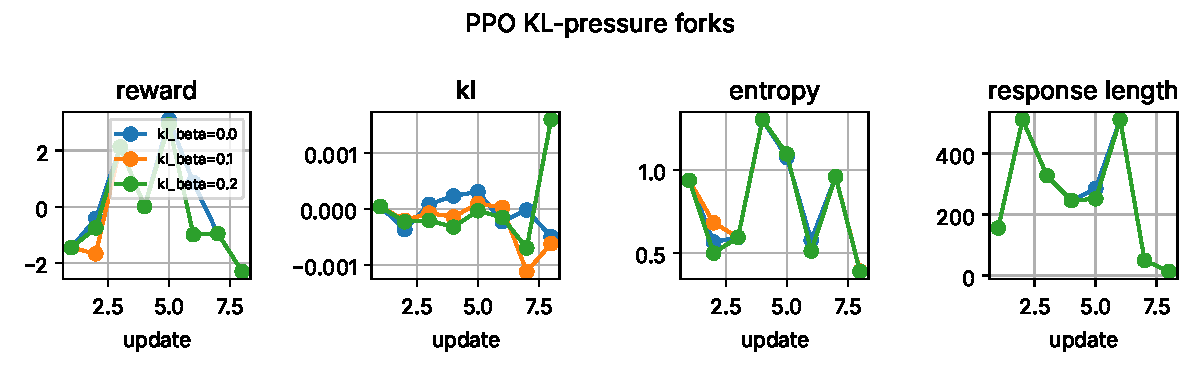
\includegraphics[width=0.9\linewidth]{kl_fork_trajectories.pdf}
\caption{Per-update trajectories of the standard PPO continuation (20 updates), the standard GRPO continuation (20 updates, $K=4$) and the PPO KL-pressure forks (8 updates).}
\label{fig:trajectories}
\end{figure}



\end{document}